\newpage
\section{Metodologia Experimental}

\subsection{Materiais}
O material utilizado para o modulador FSK foi:
\begin{itemize}
\item Módulo MCA 8801 - DataPoll;
\item Osciloscópio digital de dois canais;
\item Gerador de funções;
\item Protoboard e alicates.\\
\end{itemize}

Para o demodulador, foi empregado:
\begin{itemize}
    \item 01 Chave de fenda de 1/8”;
    \item 01 CI LM565;
    \item 01 Cl CA3140;
    \item 01 Trimpot Multivolta de 1 K$\Omega$;
    \item 02 Resistores de 560 $\Omega$;
    \item 02 Resistores de 1 $\Omega$;
    \item 03 Resistores de 3,3 $\Omega$;
    \item 01 Capacitor de poliéster de 1 nF;
    \item 05 Capacitores de poliéster de 22 nF;
    \item 02 Capacitores eletrolíticos de 100 $\mu$F / 25V.
\end{itemize}

\subsection{Métodos}

\subsubsection{Modulador FSK}

\begin{enumerate}[label=\Roman*]
    \item O circuito da Figura \ref{fig:mca8801} é um modulador FSK construído com o XR2206. O módulo MCA 8801 já possui um circuito similar a este. Estude a folha de dados do CI XR2206.
    
    \item Ainda sem o sinal de dados (banda base), calibre o modulador FSK (FM) para 10 kHz e tensão de pico de 1$V_p$ utilizando os potenciômetros. Esta será a frequência central da onda portadora.
    
    \item A conexão de uma onda quadrada na entrada do modulador FSK irá simular um trem de pulsos ”0” e ”1”, sucessivos, para os dados. Este sinal deverá ser do tipo NRZ (Non-Return-to-Zero):
    
    \begin{enumerate}[label=\alph*]
        \item com o osciloscópio, calibre o gerador de funções para saída em onda quadrada, frequência de 1kHz, e tensão de 400 $mV_p$, sem offset, i.e. sem nível DC e com razão cíclica de 50\%.
    \end{enumerate}

    \item Deve-se observar e registrar o deslocamento de frequências em resposta à onda quadrada na entrada. Passos:
    
    \begin{enumerate}[label=\alph*]
        \item Conecte o sinal modulante ajustado anteriormente no gerador de funções na entrada do modulador FSK. Quais são as duas frequências de
        saída do circuito modulador para este nível de tensão?
        
        \item Repita o item anterior alterando a amplitude do sinal do gerador na faixa de [400, 360, 320, ..., 0] mV . Registre as frequências de saída correspondentes do circuito modulador?
        
        \item Com estas medidas, determine a(s) região(ões) de operação do modulador FSK, isto é, a faixa de tensão (valores $\ge$ 0V ) modulante de entrada tal que resulte no chaveamento das frequências de saída. Quais são estas frequências?
        
        \item Para o modulador FSK circuito e tensões modulantes de entrada especificadas anteriormente é possível obter uma relação linear (Kc) entre tensão modulante e frequência modulada? Por que?
        
        \item Existe descontinuidade de fase no sinal FSK modulado (pino 2 do C.I. XR-2206, Figura \ref{fig:mca8801})?
    \end{enumerate}  
\end{enumerate}

\begin{figure}[H]
    \centering
    \caption{Circuito modulador BFSK.}
    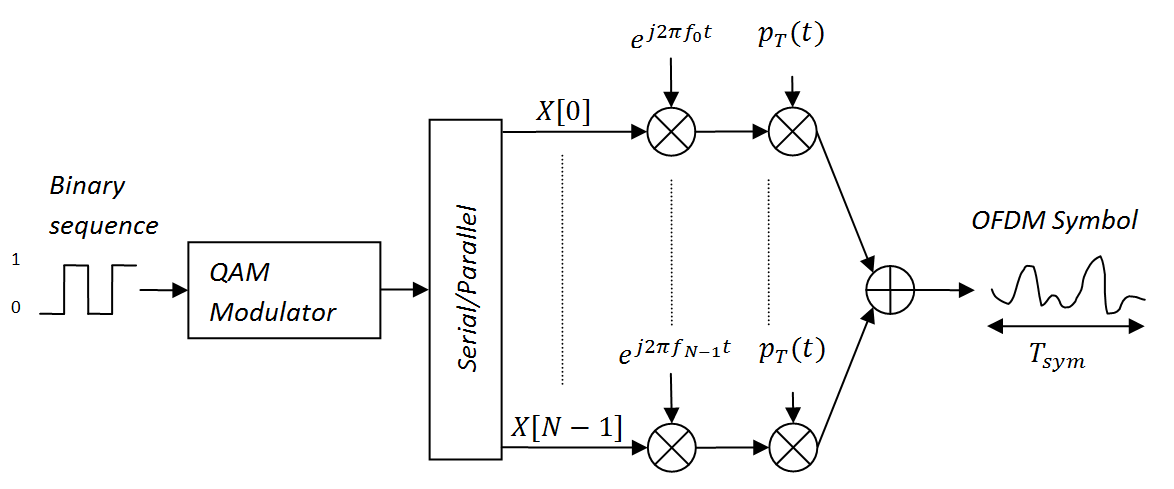
\includegraphics[scale=1.5]{mod}
    \label{fig:mca8801}
    
    \small Fonte: Me. Jaime Laelson Jacob, 2016.
\end{figure}

\subsubsection{Demodulador FSK}

Nesta etapa da experiência será analisado um demodulador FSK, parte integrante de qualquer receptor digital FSK. Um sistema de comunicação de dados em banda
base e na ausência de efeitos de canal (ruído AWGN e efeitos de desvanecimento) pode ser obtido conectando-se a saída do modulador diretamente ao demodulador.
Isto será feito a seguir.

\begin{enumerate}[label=\Roman*]
    \item Com o módulo desligado, monte o circuito da Figura \ref{fig:565}. O demodulador FSK é baseado no PLL integrado 565. Estude a folha de dados do CI565 em anexo.
    
    \item O circuito modulador FSK deve estar operando nas condições estabelecidas anteriormente. Se isto não estiver ocorrendo, repita os passos descritos na etapa anterior.
    
    \item Conecte o sinal FSK em banda base à entrada do circuito montado;
    
    \item Ligue o módulo e ajuste o trimpot $Rv1$ em sua posição média. Finalmente faça um ajuste fino em $Rv1$ até obter uma saída quadrada no osciloscópio (saída: sinal demodulado FSK). Este deve ser um ajuste preciso, obtendo, em um lado do sinal quadrado, a tensão +V e, no outro lado, a tensão -V. Ajuste para obter o centro exato destas duas indicações, resultando em simetria no sinal quadrado;
    
    \item No modulador, desconecte a entrada de dados e conecte ao ponto comum do circuito (GND).
    
    \begin{enumerate}[label=\alph*]
        \item Qual a frequência correspondente à saída do VCO (pino 4)?
    \end{enumerate}

    \item No modulador, agora reconecte a entrada de dados.
    
    \begin{enumerate}[label=\alph*]
        \item Quais as frequências correspondentes à saída do VCO (pino 4)? 
    \end{enumerate}
\end{enumerate}

\begin{figure}[H]
    \centering
    \caption{Circuito demodulador BFSK.}
    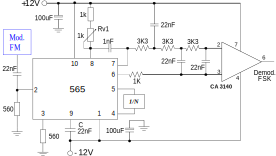
\includegraphics[scale=1.5]{demod}
    \label{fig:565}
    
    \small Fonte: Me. Jaime Laelson Jacob, 2016.
\end{figure}